\subsection{Unknown persistence: why the whole confidence set matters}\label{src16:main}
Persistence describes how strongly a source value remains related to later values. When this dependence is unknown, the test must bound how much remains after filtering. Assume a noiseless single-channel reference from a stationary Gaussian first-order autoregression, or AR(1). A centered value equals $\phi$ times its predecessor plus an independent Gaussian innovation, the new random input at that step. For $0<\phi<1$, its decay time is $-1/\log\phi\simeq1/(1-\phi)$ samples near one. Thus $(N-1)(1-\phi)$ measures record length in approximate correlation times. At $\phi=0.995$, the lengths $16385$, $32769$, and $524289$ span about $82$, $164$, and $2621$ such times.

If $\phi$ were known, the common filter $(-\phi,1)$ would remove autoregressive spectral variation. This filter subtracts the predicted part of each value and uses the same operation on both channels, leaving relative detector phase unchanged. With unknown persistence, a single fitted value cannot guarantee the required bound. We instead retain a confidence set of candidate values that are compatible with the record under a specified test. For each candidate, we compare cumulative prediction errors with their finite Gaussian distribution. The resulting two-sided set has coverage at least $0.995$: over repeated recordings, it contains the true persistence with at least this probability. Its construction, exact law, and conservative numerical cutoffs are in SM Secs.~S5.1--S5.3.

To transfer this set to the pair, both Gaussian source marginals must have the same persistence. The reference response is a nonzero scalar, the second response is a nonzero finite impulse response, and both channels are noiseless before bounded recording. Their cross spectrum is arbitrary subject to positivity and is real under the null. Independent calibration covers the unchanged second response. These assumptions connect reference information to both testing channels.

Let $[\ell,u]$ be the smallest interval containing all accepted persistence values, called the confidence hull. For $u<1$, define $\Lambda(x)=(1+x)/(1-x)$ and $z(x)=\log\Lambda(x)$. The AR(1) spectral maximum-to-minimum ratio is $\Lambda(\phi)^2$, so this transform measures the spectral variation that the covariance bound must cover. For a fixed common-filter coefficient $a$,
\begin{equation}\label{src16:placement}
 \mathcal S_a=\exp\{z(u)-z(\ell)+2|z(a)-z_c|\},\quad
 z_c=\tfrac12[z(u)+z(\ell)].
\end{equation}
The first term is uncertainty in the source. The second is the cost of placing a fixed filter away from the interval's transformed center. A wide confidence set therefore creates a large threshold even when it covers the truth and excludes one.

Let $\alpha_B$ be the source-set error, $\alpha_L$ an additional lag-set error, and $\beta$ the common energy-event failure probability.
\begin{theorem}[Source-envelope consequence]\label{src16:envelope-thm}
Assume the two-sided source set and common energy event specified in SM Sec.~S5.4, under the positive-denominator conditions stated there. On source coverage and that event, the confidence hull is nonempty, $u<1$, and
\begin{equation}\label{src16:span}
 \frac{\Lambda(u)}{\Lambda(\ell)}\le2C_{\rm gap}.
\end{equation}
The constant $C_{\rm gap}$ is explicit in the full statement in SM Sec.~S5. The probability is at least $1-\alpha_B-\beta$, or $1-\alpha_B-\alpha_L-\beta$ for the lag intersection.
\end{theorem}
In words, the stated bounds on squared fluctuations control every accepted persistence value, even if the confidence set has separate pieces. Persistence values close to one allow very slow decay and therefore large covariance bounds. Excluding one by itself only makes the envelope finite; the additional inequalities control its size. SM Secs.~S5.4--S5.5 prove the result and its correlation-time scaling. At persistence $0.8$, a target probability $0.75$ of a nonempty set excluding one requires at least $65$ differences, while $256$ suffice under error allowance $0.005$ (SM Sec.~S5.7). This factor-of-four bracket concerns endpoint exclusion, not rejection.

The test uses a finite list of filters fixed before observation. For $M$ members, the source, calibration, variance, and contrast allocations in Table~\ref{tab:budget} cover the complete union decision. A length-dependent list $a_j=1-2^{-j}$ controls placement near persistence one, whereas a fixed list bounded away from one cannot do so uniformly. SM Sec.~S5.8 gives the rule, including empty sets and unavailable members.

\subsection{A complete detection example and its observed limits}
To establish sensitivity, the preceding bounds must jointly permit rejection. The example below combines source estimation, calibration, and finite arithmetic to bound detection probability at one specified long length. Its shorter-length failures show where the same sufficient conditions remain uninformative.

\paragraph{Example: a delayed persistent source.}\label{src16:power-thm}
Let $X,Z$ be independent unit-variance Gaussian AR(1) processes with $\phi=0.995$. Observe
\[
 Y_1(t)=2+X_t,\qquad
 Y_2(t)=-1+0.9X_{t-1}+\sqrt{0.19}Z_t.
\]
Use identity responses, $N=524289$, independent 256-row two-coefficient calibration with noise standard deviation $0.01$, and the bank $(0,0.5,0.8,0.9,0.97,0.995)$. Values lie on the $2^{-20}$ grid within $2^{-21}$ of the ideal samples. Under the complete design and bounded arithmetic specified in SM Secs.~S5.9--S5.10,
\begin{equation}\label{src16:implemented-power}
 \Pr(\mathrm{reject})\ge0.91-(4N+512)e^{-128}>0.90.
\end{equation}
The full parameter statement is retained in SM Sec.~S5. The bound includes completion of all calculations needed for rejection. Earlier points on the doubling grid fail a source, variance, or contrast-margin condition; the long-record result gives no corresponding shorter-record guarantee.

The saved synthetic comparison shows how these requirements affect decisions (Fig.~\ref{fig:study-source}). Table~\ref{tab:source-outcomes} shows the transition from unavailable or inconclusive tests to detection. The lag set abstains throughout the two shorter cells because its upper endpoint still reaches one. SM Fig.~S7 locates the first failed condition, and Figs.~S1--S2 and S8 separate coverage from endpoint availability.

The improvement is conditional. At $N=8193$, the standalone set rejects $46/200$ and its split-budget intersection rejects $32/200$. Their paired difference is $0.070$, with conservative 95\% interval $[-0.006,0.142]$. At moderate persistence the intersection can instead retain detections lost by the standalone set. The two-sided threshold diagnostics at $N=524289$ have median phase allowance about $7.6\times10^{-5}$ and median sampling radius about $5.0\times10^{-4}$ (SM Figs.~S5--S6). These saved summaries show that estimating dependence remains costly even when phase calibration is accurate.

\begin{figure*}[t]\centering
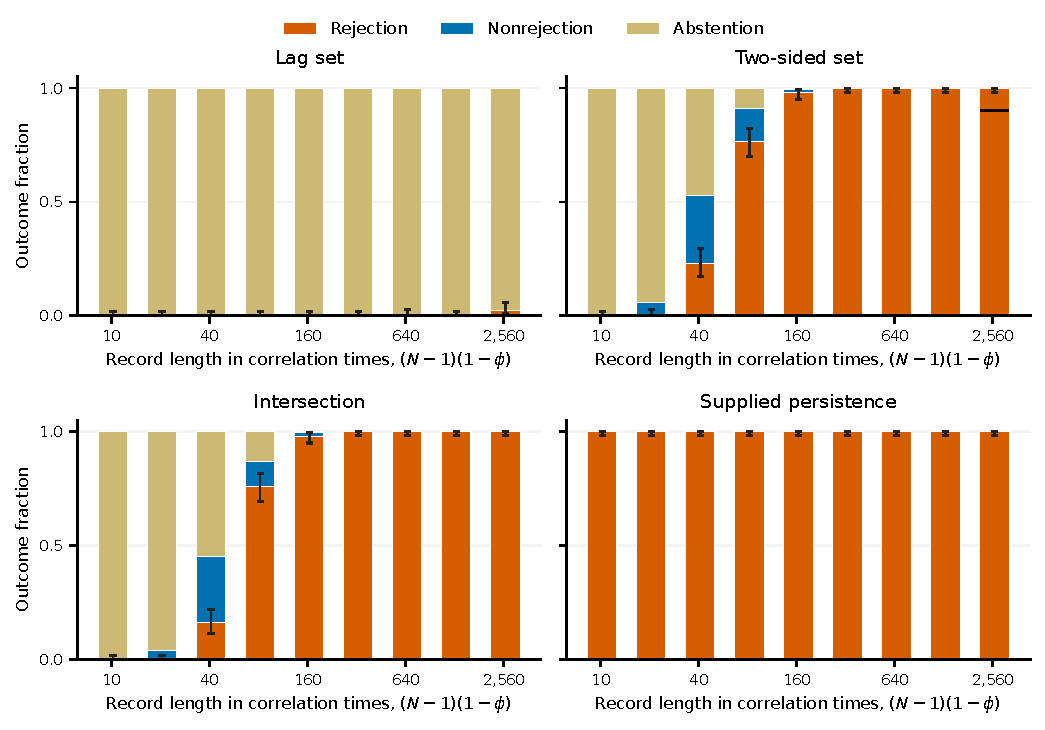
\includegraphics[width=\textwidth]{figures/source_operating_compact.pdf}
\caption{Estimating persistence delays detection even when the supplied-persistence test rejects every alternative record. Outcomes are shown against approximate correlation times $(N-1)(1-\phi)$ at $\phi=0.995$, with 200 independent records per length. Lag confidence often reaches persistence one and therefore causes abstention. Two-sided confidence becomes useful sooner; intersection is not uniformly better. Rejection intervals are pointwise 95\% binomial intervals. The ideal-model lower bound at the longest length is distinct from the observed fraction.}\label{fig:study-source}
\end{figure*}

\begin{table}[t]
\caption{Two-sided source inference at $\phi=0.995$ and strong delay. Each row uses 200 independent records. R, NR, and A denote rejection, nonrejection, and abstention.}\label{tab:source-outcomes}
\begin{ruledtabular}\begin{tabular}{rrrrr}
$N$ & $(N-1)(1-\phi)$ & R & NR & A\\
16385 & 81.92 &153&29&18\\
32769 &163.84&196&3&1\\
524289&2621.44&200&0&0\\
\end{tabular}\end{ruledtabular}
\end{table}
